\section*{Appendix B: Pauli Matrices AND Bloch Sphere}
\label{appB}
The most common operator used when it comes to requiring two eigenstates is the spin operator. The Pauli matrices form the basis for the spin operators. Here we discuss them in some more detail.

We start with the representation of a single qubit in the $\ket{0}$, $\ket{1}$ basis. $\ket{\psi}=\alpha\ket{0}+\beta\ket{1}$ with $\abs{\alpha}^2+\abs{\beta}^2=1$. Thus, the state can be represented as  $\ket{\psi} = \bigl( \begin{smallmatrix}\alpha \\ \beta\end{smallmatrix}\bigr)$. Now we can write $\abs{\alpha}=\cos\left(\bfrac{\theta}{2}\right)$ and $\abs{\beta}=\sin\left(\bfrac{\theta}{2}\right)$. The factor of half is a matter of convention. This means $\alpha=\cos\left(\bfrac{\theta}{2}\right)e^{\iota\phi_1}$ and $\beta=\sin\left(\bfrac{\theta}{2}\right)e^{\iota\phi_2}$. Since global phase does not affect observables of the system, we can factor out $\phi_1$ and set $\phi_2-\phi_1=\phi$ so that $\alpha=\cos\left(\bfrac{\theta}{2}\right)$ and $\beta=\sin\left(\bfrac{\theta}{2}\right)e^{\iota\phi}$. Thus, we can use two angular parameters, $\theta$ and $\phi$ to represent a state uniquely. These two parameters correspond to a point on a unit sphere. This sphere is called the bloch sphere, as is shown in figure \ref{Fig:Ab.1}. Note that $\theta=0$ corresponds to $\ket{0}$ and $\theta=\pi$ corresponds to $\ket{1}$.
\begin{figure}[!htb]
   \begin{minipage}{\textwidth}
     \centering
     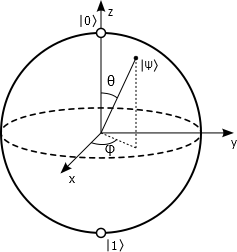
\includegraphics[scale=0.8]{figAb.01.png}
     \caption{Bloch Sphere\cite{bsphere}}
     \label{Fig:Ab.1}
   \end{minipage}
\end{figure}

Now we note that the density matrix of a state $\ket{\psi}$ in quantum mechanics can be given by $\ket{\psi}\bra{\psi}$. Thus, we write
\begin{equation}
\label{eq:Ab.1}
\begin{split}
\rho&=\ket{\psi}\otimes\bra{\psi}=\begin{pmatrix}
\cos\left(\bfrac{\theta}{2}\right)\\
e^{\iota\phi}\sin\left(\bfrac{\theta}{2}\right)
\end{pmatrix}\otimes
\begin{pmatrix}
\cos\left(\bfrac{\theta}{2}\right)&e^{-\iota\phi}\sin\left(\bfrac{\theta}{2}\right)
\end{pmatrix}\\
&=
\begin{pmatrix}
\cos^2\left(\bfrac{\theta}{2}\right)&e^{-\iota\phi}\cos\left(\bfrac{\theta}{2}\right)\sin\left(\bfrac{\theta}{2}\right)\\
e^{\iota\phi}\cos\left(\bfrac{\theta}{2}\right)\sin\left(\bfrac{\theta}{2}\right)&\sin^2\left(\bfrac{\theta}{2}\right)
\end{pmatrix}\\
&=
\begin{pmatrix}
1+\cos\theta&\cos\phi\sin\theta-\iota\sin\phi\sin\theta\\
\cos\phi\sin\theta+\iota\sin\phi\sin\theta&1-\cos\theta
\end{pmatrix}\\
&=
\bfrac{1}{2}\left(
\mathbb{I}+
\begin{pmatrix}
0&1\\
1&0
\end{pmatrix}
\sin\theta\cos\phi+
\begin{pmatrix}
0&-\iota\\
\iota&0
\end{pmatrix}
\sin\theta\sin\phi+
\begin{pmatrix}
1&0\\
0&-1
\end{pmatrix}
\cos\theta
\right)
\end{split}
\end{equation}
Now note that a unit vector on the sphere can be written, in spherical polar coordinates as $\hat{\mathbf{n}}=(\sin\theta\cos\phi,\sin\theta\sin\phi,\cos\theta)$. If we write $\mathbf{\sigma}=(\sigma_x, \sigma_x, \sigma_z)$, with
\begin{equation}
\label{eq:Ab.2}
\begin{split}
\sigma_x&=\begin{pmatrix}
0&1\\
1&0
\end{pmatrix}\\
\sigma_y&=\begin{pmatrix}
0&-\iota\\
\iota&0
\end{pmatrix}\\
\sigma_z&=\begin{pmatrix}
1&0\\
0&-1
\end{pmatrix}
\end{split}
\end{equation}
then we can modify equation \ref{eq:Ab.1} to
\begin{equation*}
\rho=\bfrac{1}{2}\left(\mathbb{I}+\hat{\mathbf{n}}.\mathbf{\sigma}\right)
\end{equation*}
The 3 matrices in \ref{eq:Ab.2} are the Pauli matrices, which are used as gates. These matrices have some interesting properties which makes solving problems easier using them, but they are not very relevant to our work and hence, we shall not discuss them here. They can be looked up from any standard textbook on quantum mechanics\cite{shankar}.